\begin{landscape}
\chapter{Листинги}
\section{Файл разметки для modbus тегов}

\lstinputlisting[
    language=XML,
    caption="modbus scheme",
    label=lst:modbus_tags_configs]
        {Dissertation/listings/modbus_tags_configs.xsd}

\end{landscape}

\chapter{Свидетельство о государственной регистрации программы для ЭВМ}\label{ch:app1}

\todo{Свидетельство и акт я получу на работе.}

\begin{center}
    \begin{figure}[hb]
        
\includegraphics[width=.7\textwidth]{registration}
        \caption{Скан свидетельства о регистрации}\label{app:fig:registration}
    \end{figure}
\end{center}
    


\chapter{Акт о внедрении}\label{ch:app2}

\begin{center}
    \begin{figure}[hb]
        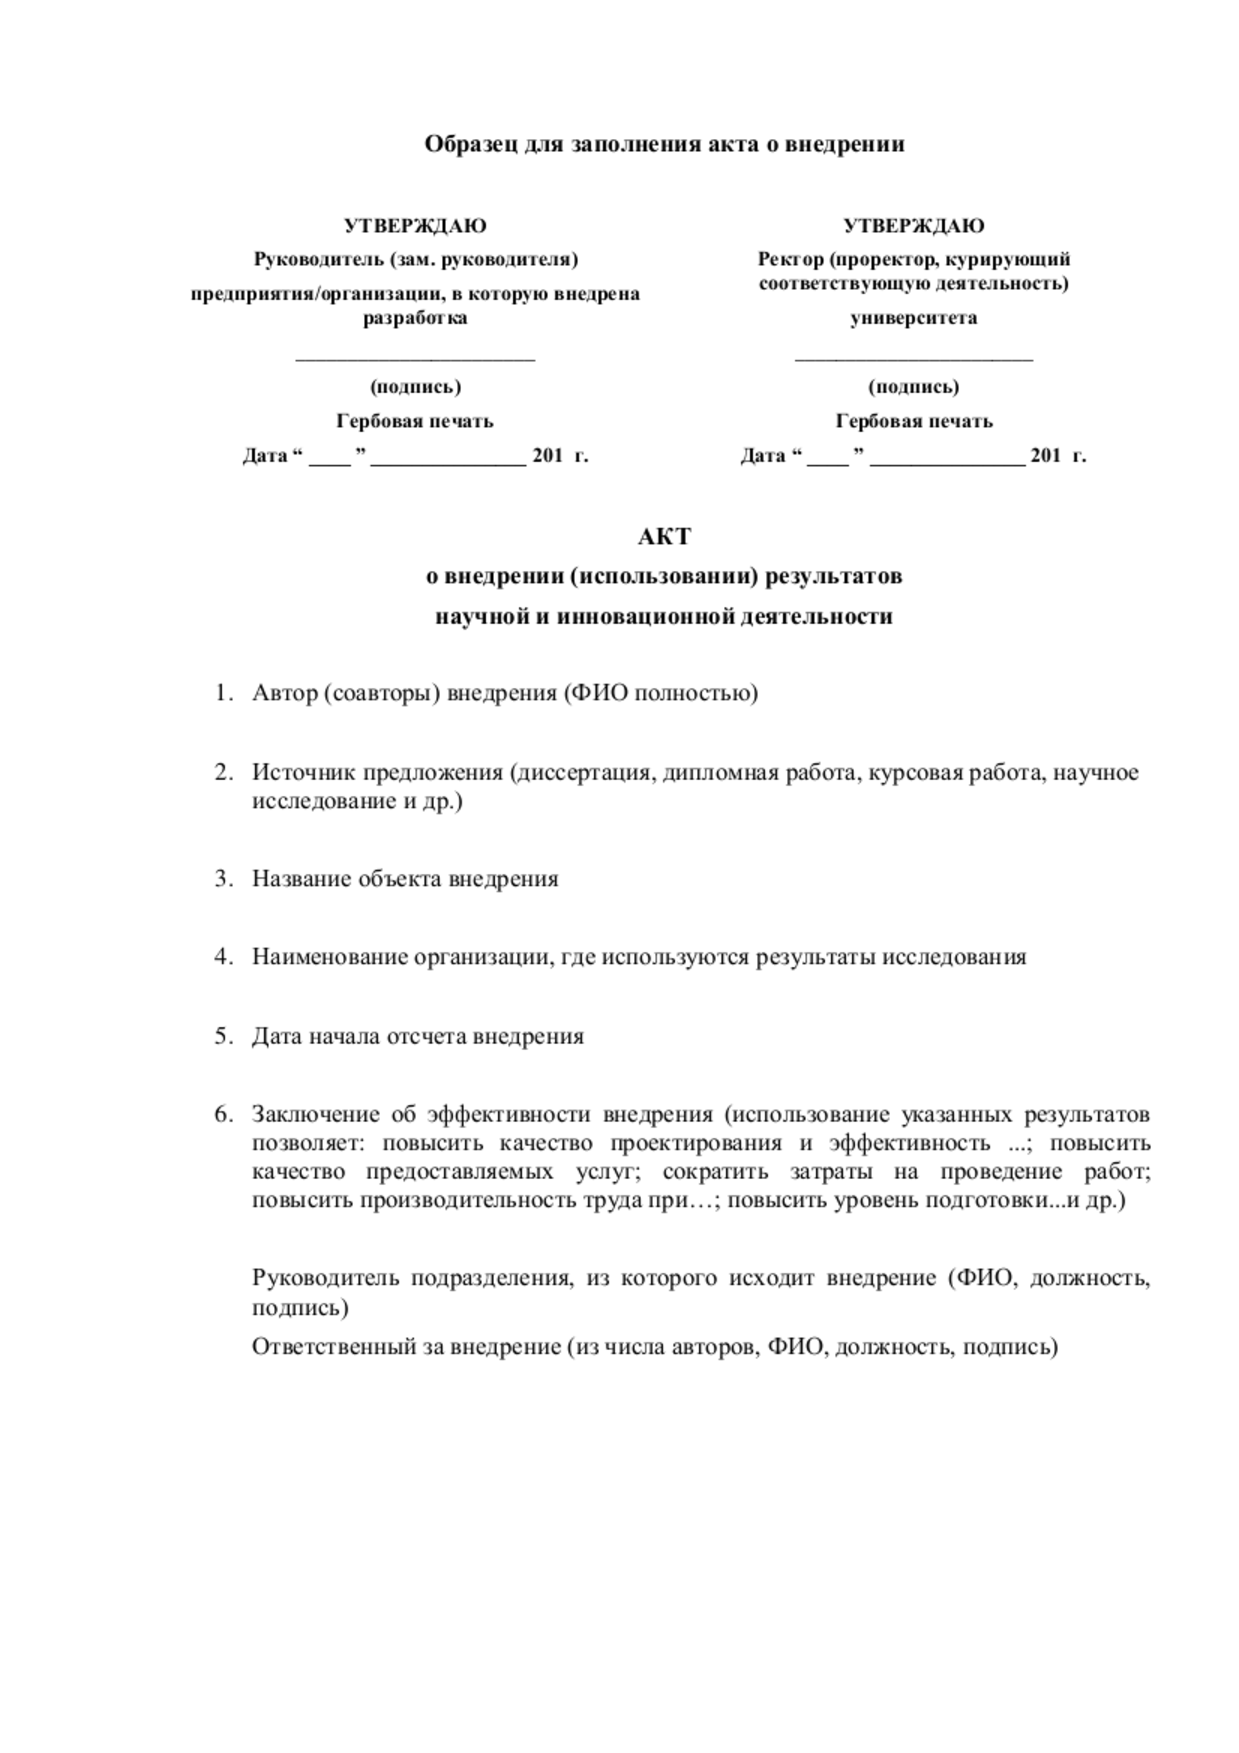
\includegraphics[width=.7\textwidth]{implementation.pdf}
        \caption{Акт о внедрении}\label{app:fig:implementation}
    \end{figure}
\end{center}